%In this laboratory activity, we implemented an open-loop camera system to stabilize a pan-tilt camera mechanism (on a TurtleBot) using IMU data. 

In this laboratory activity, we implemented an open-loop camera stabilization system on a TurtleBot using data from an Inertial Measurement Unit (IMU). The main objective was to maintain a stable field of view for a pan-tilt camera mechanism by compensating for the robot's motion. The stabilization was achieved by calculating tilt and pan angles from the BNO55 IMU sensor and driving two servo motors via the PWM signals. A proportional control strategy was adopted for simplicity and effectiveness, with no position feedback, making it a true open-loop system. Data was logged for further analysis using STM32 and MATLAB. \\
\noindent
This lab introduced key concept such as sensor-based orientation estimation, servo control via PWM, basic proportional controllers and embedded data logging.

%and optional improvement using sensor fusion.

%The exercise involved extracting motion data from the IMU, calculating the tilt and pan angles, and using servo control through PWM signals to realign the camera accordingly. 

\subsection{Problem Analysis}

As TurtleBot moves, its body tilts and pans, causing the camer mounted on the robot to lose its horizontal alignment. This affects the video feed's usability and clarity. The goal is to counteract these motions by adjusting the camera's orientation, ensuring that it remains level with the ground. The key tasks include: 

\begin{itemize}
    \item measuring the robot's motion via accelerometer and gyroscope data.
    \item calculating corresponding tilt (pitch) and pan (yaw) angles.
    \item generating PWM signals to actuate the servo motors and realing the camera.
\end{itemize}

Because the control is open-loop, the system does not read back the actual servo position, so relying on estimated orientation from the IMU.



% USE SENSOR INPUT TO CONTROL SERVO ANGLES FOR CAMERA STABILIZATION
% THE AIMS ARE ESTIMATING ANGLES ACCURATELY USING ACCELEROMETER AND GYROSCOPE DATA, CORRECTLY MAPPING CONTROL SIGNAL TO SERVO PWM VALUES,
%OPERATING WITHOUT FEEDBACK


% When the TurtleBot rotates along the x-axis, the camera tilts with the robot, disrupting a stable wiev. The task is to design a open-loop controller that automatically adjust the tilt servo to counteract the motion and keep the camer level with the horizon. Sensor data from the accelerometer and gyroscope must be processed to derive the current tilt angle and apply corrective control signals to the servo motor.



\subsection{Theoretical background}


%% SPIEGARE METODI PER IL CALCOLO DEL TILT E PAN ANGLE
%% COME MUOVERE LA TELECAMERA CON PWM

\subsubsection{Orientation estimation using IMU}

%BNO55 provides accelerometer and gyroscope data and is used to acquire motion data via I2C. Communication wrappers for reading and writing register are defined using HAL function. 
%bno55_convert_double_accel_xyz_msq()
%bno55_convert_double_gyro_xyz_rps()


From the IMU data, we derive the pitch (tilt) angles, used to orient the camera. There are two main methods used to estimate these angles: 

\begin{itemize}
    \item \textbf{Accelerometer-Based Tilt Estimation}
    
\end{itemize}

\noindent
For the first method we use the y-axis acceleration to compute tilt:

\[\theta = \sin^{-1} \left(\frac{a_y}{g}\right) \]

where $\theta$ is the tilt angle, $a_y$ is the y-acceleration (m/$s^2)$ and $g=9.81 $ $m/s^2$ is the gravitational acceleration.
\noindent
This method is effective for low-frequency, static measurements, but is sensitive to noise and external acceleration.

\bigskip
\begin{itemize}
    \item \textbf{Gyroscope-Based Tilt Estimation}
    
\end{itemize}
\noindent
Instead, if we use this second method, the angular velocity $\omega_x$ from the gyroscope is integrated over time to estimate the tilt angle displacement:

\[\theta_g(t) = \int \omega_x(t) \, dt\]

Then we need to convert it to degrees by multiplying it by 180/$\pi$.

This method accumulates angular displacement over time but suffers from drift due to bias in the gyroscope. 


\subsubsection{Pulse Width Modulation (PWM)}

%Pulse Width Modulation (PWM) is a technique used to simulate analog voltage levels by varying the duty cycle of a digital pulse signal.

Pulse Width Modulation (PWM) is a technique used to simulate analog output using digital signals.
Instead of delivering a constant voltage, PWM controls the amount of power delivered to a device by rapidly switching the signal between high and low states. The key parameter is the duty cycle, which represents the proportion of time the signal stays high within each period.

For example, if the PWM signal has frequency of 50 HZ (i.e. a period of 20 ms), a duty cycle of 50\% means that the signal is high for 10 ms and low for 10 ms within each cycle. By adjusting this ratio, it is possible to control how much effective power is delivered to a device, such as servo motor. 

PWM is widely used embedded systems because it provides an efficient way to control actuators without the need for digital-to-analog converters (DACs). In practice, STM32 hardware timers are configured to generate PWM signals with precise timing and frequency, ensuring stable and responsive control.


%% IMU E SERVO MOTOR

\subsection{System Configuration}

\subsubsection{IMU}


An IMU (Inertial Measurement Unit) is an electronic component used to measure and report an object's linear acceleration, angular velocity and orientation in 3D space. Specifically, we have used: 

\begin{itemize}
    \item a 3-axis accelerometer, which measures linear acceleration along the x, y and z axes.
    \item a 3-axis gyroscope, which measures angular velocity around the same axes.
\end{itemize}

\noindent
These axes are aligned as follows: 

\begin{itemize}
    \item \textbf{x-axis}: pointing to the right
    \item \textbf{y-axis}: pointing backward
    \item \textbf{z-axis}: pointing downwards (towards the ground)
\end{itemize}
%--> TURTLEBOT AXES X, Y, Z

%IMU is equipped with a 3-axis accelerometer that measures linear acceleration and a 3-axis gyroscope that measures the angular velocity in rad/s. 

%HOW IT WORKS ACCELEROMETER AND GYROSCOPE 
\noindent
From the IMU data, we derive the standard Euler angles used in orientation estimation: 

\begin{itemize}
    \item \textbf{Pitch}(Tilt): rotation around the x-axis.
    \item \textbf{Roll}: rotation around the y-axis.
    \item \textbf{Yaw} (Pan): rotation around the z-axis.
\end{itemize}

In our lab setup, tilt refers to the vertical rotation of the camera (pitch), and pan refers to the horizontal rotation (yaw). 

\subsubsection{Servo motor via PWM}

%In this lab, two servo motors were used: one for vertical (tilt) and one for horizontal (pan) adjustment. These servos are controlled through PWM signals generated by the STM32 microcontroller.

In this laboratory, PWM was used specifically to control the position of two servo motors, one for adjusting the til and the other for the pan of a camera mounted on the TurtleBot. Unlike regulare DC motors, which rotate continuously, servos rotate only to a commanded position within a limited range, such as -45° to +45°.

Servo motors interpret PWM signals to determine their target angle. The control signal consists of a PWM signal at a constant frequency, where the pulse width determines the desired angle.

This means the servo expects a PWM signal with a fixed period, where only the duration of the high signal varies. 

To control the servos in our system, we used 
the STM32's Timer 1, which support multiple channels for independent signal generation. 

In this lab setup:

\begin{itemize}
    \item Tilt (Pitch) Servo is connected to TIM1, Channel 3
    \item Pan (Yaw) Servo is connected to TIM1, Channel 2
\end{itemize}

These channels are mapped to specific GPIO pins configured for alternate function mode (AF), enabling them to output the PWM signal generated by TIM1. 

%HAL_TIM_SET_COMPARE()
%saturate()

%The parameters of the PWN and the min and max servo angles were already configured to respect the mechanical constraints without damaging the servos.  
%The PWM is generated using TIM1 and in particular, the tilt is controlled by CHANNER\_3 of TIM1 while the pan is controlled by CHANNEL\_2.

%TO move the camera, we used the following HAL functions:...

%\_\_HAL\_TIM\_SET\_COMPARE is used for setting the compare value for channel 2 and 3 of the TIM1 hardware timer. 



\subsection{Code implementation and Control}

\subsubsection{Tilt Control}

Accelerometer and gyroscope data are read using: 

\begin{lstlisting} [language=C]
bno055_convert_double_accel_xyz_msq(&d_accel_xyz); 
bno055_convert_double_gyro_xyz_rps(&d_gyro_xyz);
\end{lstlisting}

A proportional controller was used to compute the tilt control signal:

\begin{lstlisting} [language=C]

float a_y;
float g = 9.81f;
float K_p_tilt = -1;
float theta_a = 0;

theta_a = asin(a_y/g) * 180.0 / M_PI;// [deg]

tilt = K_p_tilt * theta_a;

\end{lstlisting}


The control signal is then applied to the tilt servo using: 

\begin{lstlisting} [language=C]
_HAL_TIM_SET_COMPARE(&htim1, TIM_CHANNEL_3,(uint32_t)saturate((150+tilt*(50.0/45.0)), 
SERVO_MIN_VALUE, SERVO_MAX_VALUE)); // tilt
\end{lstlisting}

The calculated angle \texttt{tilt} is first scaled to match the corresponding PWM value. This involves mapping the angular range to a range of timer-comparison values that corresponds to the pulse width.  

The mapping used in this laboratory is: 
\begin{lstlisting} [language=C]
(uint32_t)(150+tilt*(50.0/45.0)
\end{lstlisting}

where 150 represents the neutral position, tilt the control input in degrees and 50/45 is a scaling factor to convert $\pm 45$° to $\pm 50$ PWM units. 

To ensure safety, this value is passed through a saturate() function that clamps it within the physical limits of the servo, preventing over-rotation or mechanical damage. 

%The tilt and pan control signals are derived as follows: \\

-- INSERT CODE





\subsubsection{Data logging}

Data logging uses either:

\begin{itemize}
    \item Serial interface via USB (use in this lab)
    \item Wifi datalogger 
\end{itemize}


The matlab commands used to visualize the logged data are:

\begin{lstlisting} [language=matlab]
data = serial_datalog ('COMx', {'3*single','1*single'}, 'baudrate', 115200);
\end{lstlisting}

where 3*single represent accelerometer readings and 1*single the control signal.


The C data structure for logging

\begin{lstlisting} [language=C]

struct datalog
{
    //float accel_x, accel_y, accel_z;
    //float gyro_x, gyro_y, gyro_z;
    float th, control_signal_tilt;
    float ph_g, control_signal_pan;
} logger_data;

\end{lstlisting}

Logging in the main loop:

\begin{lstlisting} [language=C]


    logger_data.accel_x = d_accel_xyz.x;
    logger_data.accel_y = d_accel_xyz.y;
    logger_data.accel_z = d_accel_xyz.z;
    logger_data.gyro_x = d_gyro_xyz.x;
    logger_data.gyro_y = d_gyro_xyz.y;
    logger_data.gyro_z = d_gyro_xyz.z;*/
    
    logger_data.control_signal_tilt = tilt;
    logger_data.control_signal_pan = pan;
    logger_data.th = theta_a;
    logger_data.ph_g = phi_g;
    
    ertc_dlog_update(&logger);//check if some one is connected and waiting for data
    ertc_dlog_send(&logger, &logger_data, sizeof(logger_data));//send data A MATLAB

\end{lstlisting}


\subsection{Results}

Exercise 1 - develop a control law to stabilize the camera's tilt by utilizing data from an IMU.

\subsubsection{Exercise 1 : Tilt Stabilization}

Using the accelerometer-based tilt estimate and a proportional controller, the camera sussfully maintained a level tilt when the TurtleBot was manually tilted forward and backward. The servo responded proportionally to the calculated angle, demonstrating a functioning open-loop stabilization.


\begin{figure}[H]
    \centering
    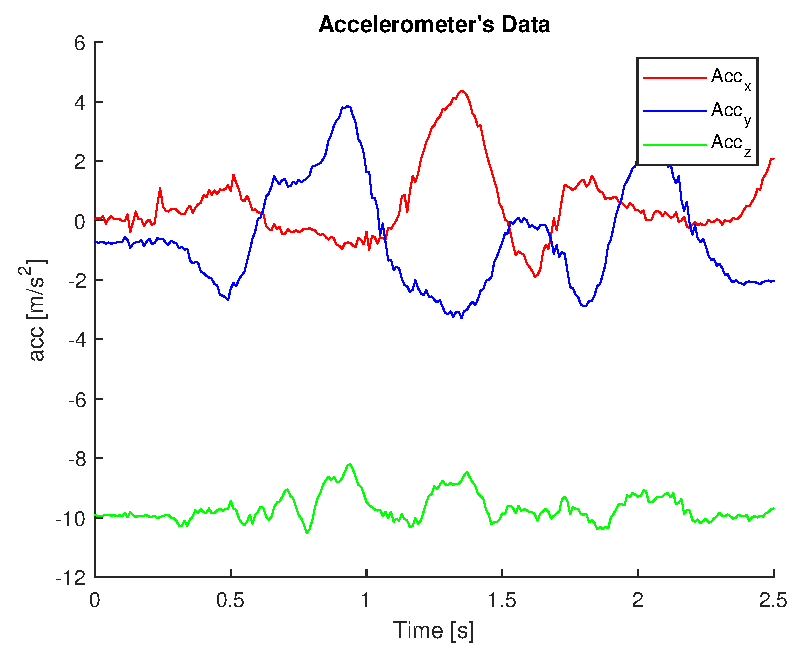
\includegraphics[width=0.5\linewidth]{lab1-2/figures/Accelerometer_Data.eps}
    \caption{Accelerometer data}
    \label{fig:acc_data}
\end{figure}

\begin{figure}[H]
    \centering
    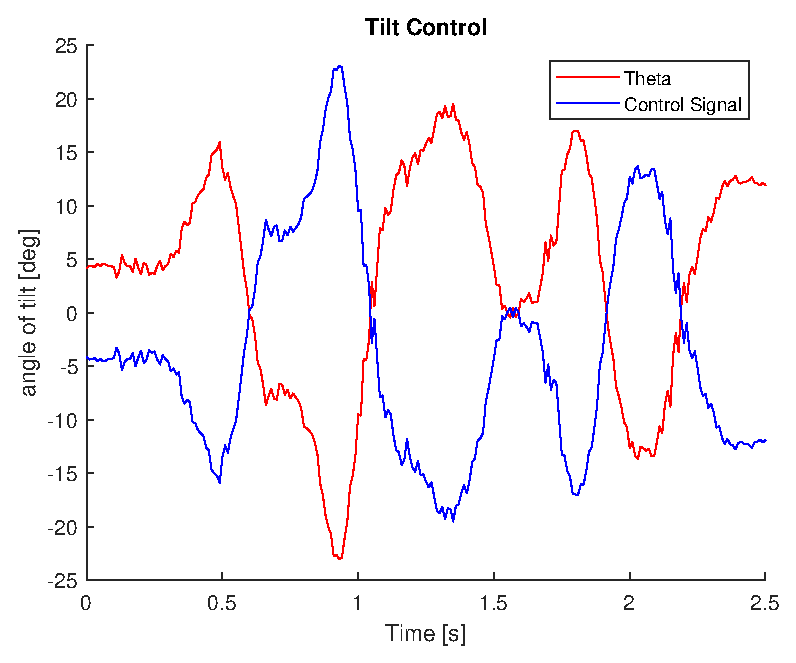
\includegraphics[width=0.5\linewidth]{lab1-2/figures/Tilt.eps}
    \caption{Tilt}
    \label{fig:tilt}
\end{figure}



--- ADD PLOT AND VIDEOS

\subsubsection{Bonus: Smooth Pan Control}

Bonus 1 - control algorithm that implements a "smooth pan" control using data from the gyro.  \\

The pan control using gyroscope data produced a smooth response. Since yaw changes accumulate over time, the camera followed the turning motion of the TurtleBot with a lag defined by the proportional gain.








